% Chapter Template

\chapter{Context} % Main chapter title

\label{Chapter2} % Change X to a consecutive number; for referencing this chapter elsewhere, use \ref{ChapterX}

%----------------------------------------------------------------------------------------
%	SECTION 1
%----------------------------------------------------------------------------------------

\section{Mutation Testing}

Mutation testing is a testing technique which consists on modifying an application (by injecting bugs) in order to enhance and evaluate the quality of the test suite that accompanies it. Each injected bug generates a new version of the application, and its called \textbf{mutant}. Each mutant differs from the original version in a simple modification, called \textbf{mutation}. As an example, if there is a compound logical operation in the original version, a valid mutation consists in replacing one and only one of the logical operators in the compound operation (i.e. if there is an "AND", the mutation changes  it with "OR"). It is worth noticing, that the replacement of each operator in the compound operation generates one mutant.

Now, to determine how many mutants can be generated, mutation testing uses a set of rules called \textbf{mutation operators} that define common errors and practices that belong to programming rules (e.g., replace a math operator ), or to the specific programming language context (e.g., assign a null value to an Intent parameter ). Therefore, depending on the tool used to generate the mutants, the application to be mutated is analyzed to derive a Potential Fault Profile \cite{linares2017enabling,Moran:ICSE18}, i.e., a set of possible locations where a mutant operator can be applied. For each of this locations the mutation tool creates a copy of the original app, and this copy is a modification produced by applying a mutation operator. Several mutation operators have been proposed for different types of applications such as web apps \cite{praphamontripong2016experimental}, data-centric apps \cite{appelt2014automated}, NodeJS packages \cite{rodriguez2018mutode} and Android apps \cite{linares2017enabling}. Table \ref{table:mtpfsc} summarizes different implementations of mutation testing in several programming languages and for different types of applications.

For more information about mutation testing you can refer to Chapter 5 of Paul Ammann and Jeff Offutt book called Introduction to Software Testing \cite{ammann2016introduction}, or the survey by Jia and Harman \cite{Jia:TSE11}.

\begin{table}[H]
	\centering
		\caption{Mutation testing papers for different application types.}
	\label{table:mtpfsc}
	\begin{tabular}{|p{3cm} | p{10cm}|} 
		\hline
		App type/Language & Paper \\ [0.5ex] 
		\hline\hline
		Java & Yu-Seung Ma, Yong Rae Kwon, and Jeff  Offutt. 2002. \textbf{\textit{Inter-Class Mutation Operators for Java.}} In 13th International Symposium on Software Reliability Engineering (ISSRE’02) \\
		\hline\hline
		Python & Anna Derezinska and Konrad Halas. 2014. \textbf{\textit{Analysis of Mutation Operators for the Python Language.}} Proceedings of the Ninth International Conference on Dependability and Complex Systems (DepCoS14) \\ \hline\hline
		Web Apps & Upsorn Praphamontripong, Je  Outt, Lin Deng, and Jingjing Gu. \textbf{\textit{An Experimental Evaluation of Web Mutation.}} ICSTW’16 \\ \hline\hline
		Data-Centric Apps & Dennis Appelt, Cu Duy Nguyen, Lionel C. Briand, and Nadia Alshahwan.\textit{ \textbf{Automated testing for SQL injection vulnerabilities: an input mutation approach.}} ISSTA’14 \\ \hline\hline
		GUIS & R. A. P. Oliveira, E. Alégroth, Z. Gao, and A. Memon. \textbf{\textit{Definition and evaluation of mutation operators for GUI-level mutation analysis.}} ICSTW’15 \\ \hline\hline
		Test Data & Daniel Di Nardo, Fabrizio Pastore, and Lionel C. Briand. 2015. \textbf{\textit{Generating Complex and Faulty Test Data through Model-Based Mutation Analysis.}} ICST’15 \\
		\hline\hline
		Android & Mario Linares-Vásquez, Gabriele Bavota, Michele Tufano, Kevin Moran, Massimiliano Di Penta, Christopher Vendome, Carlos Bernal-Cárdenas and Denys Poshyvanyk. 2017. \textit{\textbf{Enabling Mutation Testing for Android Apps}}. ESEC/FSE 2017 \\
		\hline\hline
		NodeJS & Diego Rodríguez-Baquero, and Mario Linares-Vásquez. 2018. \textit{\textbf{Mutode: generic JavaScript and Node. js mutation testing tool}}. ISSTA 2018 \\
		\hline
	\end{tabular}
\end{table}


\section{Android App Building Process}

In order to understand some of the problems and design decisions  in this thesis, it is important to know how android applications are built from the source code into an Android Application Package ( APK ), which is the file deployed to an Android device. It is worth noticing that Android applications can be developed in several ways, whether using first-class languages\footnote{text} as JAVA, Dart or Kotlin, or using frameworks for cross-platform development (e.g. Ionic, Phonegap, React4Native). Nevertheless, native approaches generates a project in a first-class language to be deployed in mobile devices. Therefore, for the purpose of this explanation lets assume the application to study was developed using a first-class (i.e., native) language. 

Resource files (i.e., color.xml, strings.xml, etc.), application files (e.g, *.java) , libraries  (i.e, jar files) and the Android manifest file are packaged in an APK file. The process starts with compiling the app source code to java bytecode, and then compiling bytecode  and libraries to dex code. Dex code is the set of operations that are going to be executed by the VM in an Android device. Previously generated files along with the already compiled libraries are compiled using the  \textit{dx} tool into one or several .dex files\footnote{For more information about multidex visit: \url{https://developer.android.com/studio/build/multidex?hl=es-419}}. Finally, packaged resource files and dex file(s) are packaged into an unsigned apk. So, while Java, Kotlin and Dart are high-level languages, dex operates as an intermediate representation that is closer to the machine.

\begin{figure}[h!]
	\caption{Android Building process.}
	\centering
	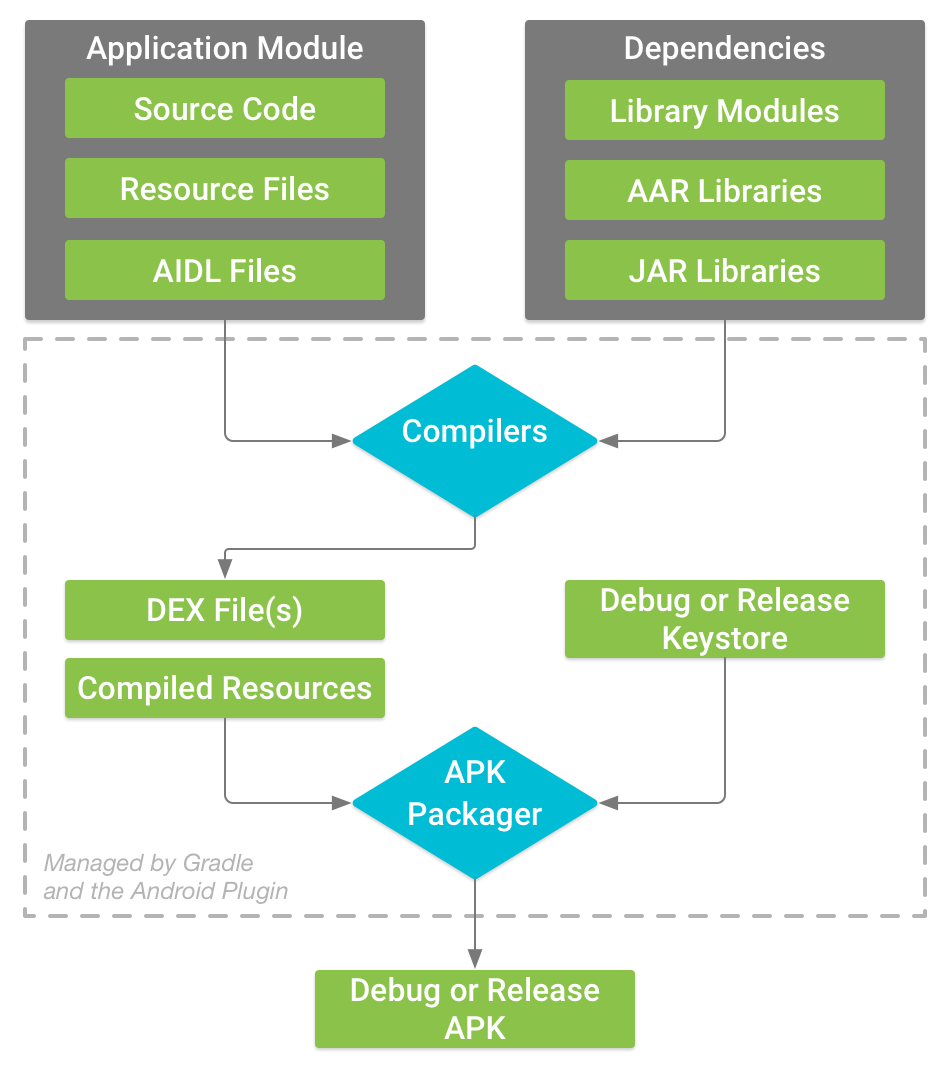
\includegraphics[width=0.7\textwidth]{../Figures/android-build-process.png}
	\label{fig:abp}
\end{figure}


\section{Intermediate Representations (IR)}

An intermediate representation is a representation of the source code aimed at being more expressive  and easier of interpretation for a machine. An intermediate representation has the property that without losing app behavior, it presents the source code in a less complex format or in a less cumbersome context, from the point of view of a machine. In the specific case of Android apps, there are several intermediate  representation; we will briefly describe 4  of the them, that have been widely used in research.:  Java Bytecode, Dex, Smali, and Jimple. The first two are the closer representations to the starting and ending point of the Android application building process, while the other two (even being closer to the endpoint) have been created with the purpose of enabling analysis tasks on the source code. 

One of the benefits of using intermediate representations (in the context of JAR and APK analysis) is avoiding the decompilation of the app to reach the original source code; in the specific case of Android apps, by using an intermediate representation we get rid of reversing the android building process.

\subsection{JAVA Bytecode}

This intermediate representation is used by the Java Virtual Machine (JVM). It is worth noting that JVM follows a stack-based architecture \cite{jvms}. The most common way to get into this representation is through JAVA itself. However, there are compilers for other languages and frameworks into Java Bytecode. For example, SCALA, Clojure, Object Pascal, Kotlin and others \cite{pljvm}. As presented previously, Java Bytecode is the first resulting representation when compiling an android application source code.

\subsection{Dalvik Bytecode (DEX)}

Originally designed to work with Dalvik VM (DVM) and the Android Runtime (ART), the dalvik bytecode was designed for systems as mobile devices that have restrictions in their computational power \cite{dvmi, jitcadvm}. Actually, the Dalvik VM has been replaced by the Android Runtime (ART) keeping the same dalvik bytecode as representation to its execution. It is worth noting  that both DVM and ART follow a register-based architecture that normally requires fewer, but typically more complex VM instructions.

\subsection{JIMPLE}

Jimple is an intermediate representation used by Soot \cite{soot}. Jimple is based in 15 different operations that compared with the over 200 operations defined for Java bytecode makes it easier to optimize, however a lot of information can be lost when translated from java bytecode to Jimple.

\subsection{SMALI}

SMALI is an intermediate representation created by Ben Gruver \cite{smali}. It offers a readable version of the Dalvik bytecode, due to the similar amount of operations supported for both representations. As it is closer to dalvik bytecode rather than Java bytecode it represent the code following a register-based architecture. This enhances our possibilities to analyze applications because all Java instructions tend to be separated from recursive calls. For example, if a new object is created inside the parameter field of a method, SMALI translates the object creation into one line and the method call into another as it can be seen in Figure \ref{fig:sre}. Because of this, as it will be seen in next sections, we were able to recognize more potential fault injection points that are more complex to be recognized when analyzed in Java.

\begin{figure}[H]
	\caption{SMALI representation example}
	\centering
	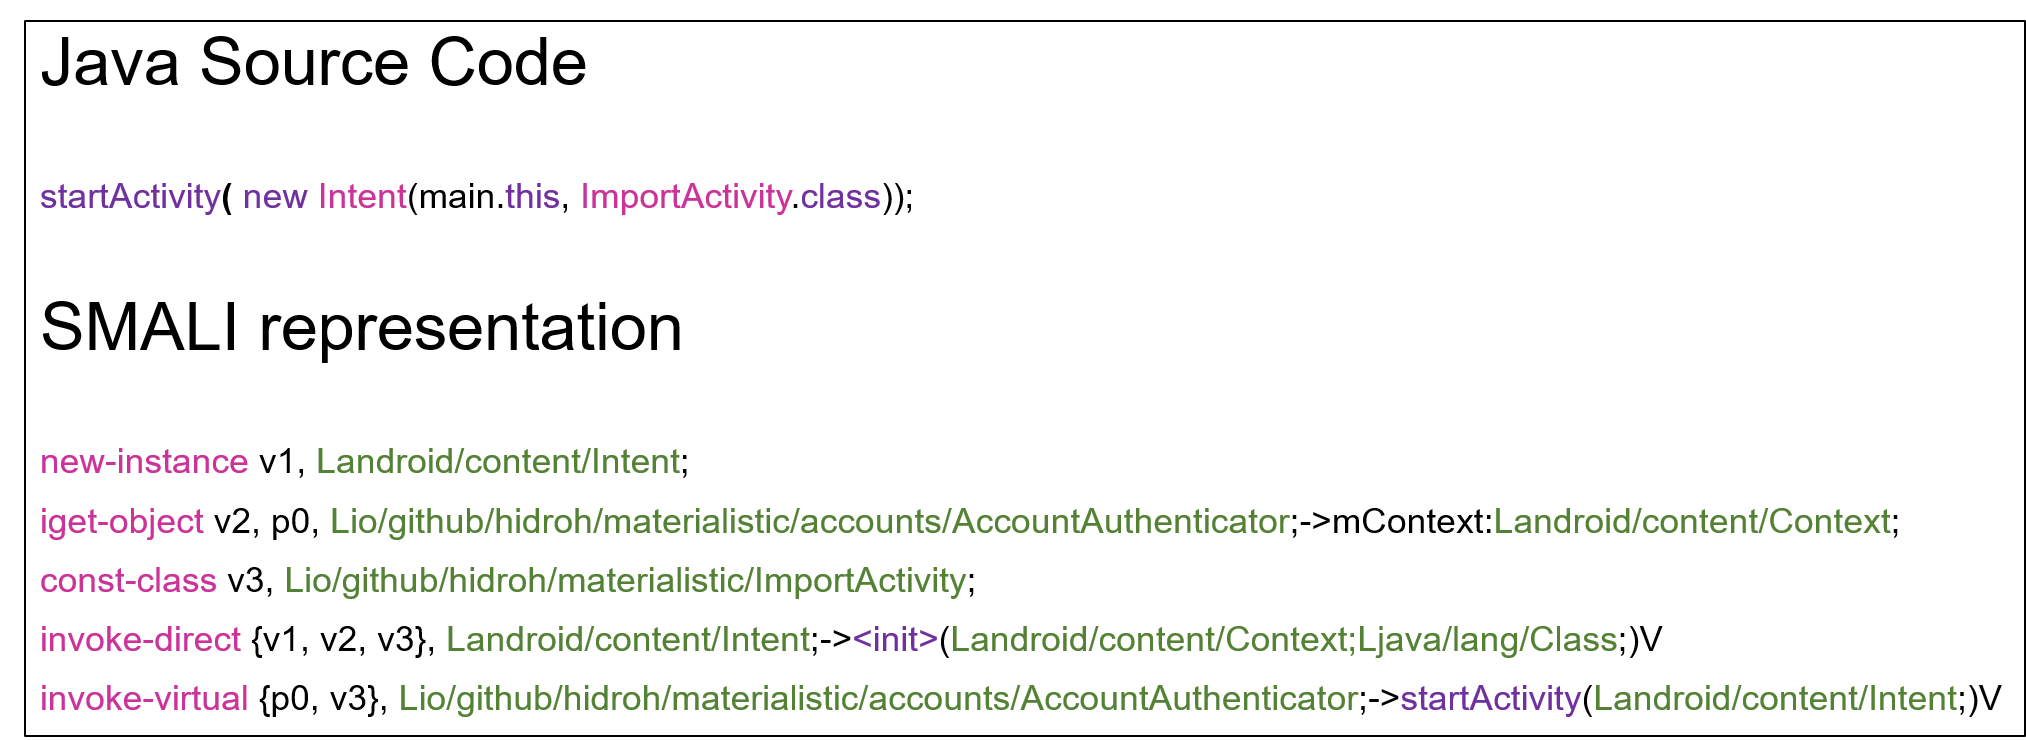
\includegraphics[width=\textwidth]{../Figures/smali}
	\label{fig:sre}
\end{figure}


